\documentclass[a4paper,11pt]{elsarticle}
\usepackage{graphicx}
\usepackage{amsmath}
\usepackage{amssymb}
\usepackage{natbib}
\usepackage{caption}
\usepackage{subcaption}
\usepackage{multicol}
\usepackage{color}
\usepackage{xspace}
\usepackage{enumerate}

\newtheorem{theorem}{Theorem}
\newtheorem{definition}[theorem]{Definition}

\bibliographystyle{elsarticle-num}

\title{A Differential Geometric Approach to Time Series Forecasting}

\author[1]{Babak Emami\corref{cor1}%
\fnref{fn1}}
\ead{babak.emami@gmail.com}
\cortext[cor1]{Corresponding author}
\fntext[fn1]{The author is an independent researcher.}
\address[1]{1335 Filbert St., 303, San Francisco, CA, United States 94109}

\begin{document}

\begin{abstract}
  
A differential geometry based approach to time series forecasting is
proposed. Given observations over time of a set of correlated
variables, it is assumed that these variables are components of
vectors tangent to a real differentiable manifold. Each vector belongs
to the tangent space at a point on the manifold, and the collection of
all vectors forms a path on the manifold, parametrized by time. We
compute a manifold connection such that this path is a geodesic. The
future of the path can then be computed by solving the geodesic
equations subject to appropriate boundary conditions. This yields a
forecast of the time series variables.

\end{abstract}

\begin{keyword}
time series \sep forecast \sep manifolds \sep geodesic
\end{keyword}

\maketitle

\section{Introduction}\label{section:introduction}

Forecasting of time series arises in various fields, such as economics
\cite{kennedy-1998, fabozzi-etal-2014}. The conventional approach is
to regress the response time series, that is the dependent variable,
against the time series of a set of variables which are called
predictors or independent variables. The choice of regression model
depends on the nature of relationship between response and predictors
and can be selected from a wide range of models including linear
regression, neural networks, and kernel methods such as the Gaussian
process
regression~\cite{hastie-etal-2009,rasmussen-williams-2005}. Once the
parameters of a model are estimated, the future of response can be
calculated given the future values of predictors.

There are two issues with the above-mentioned approach. First, the
future values of predictors are needed to forecast response. In most
cases, future values of predictors are not known, making the forecasts
dependent on potentially inaccurate estimations. For example in
economics, the macro-economic indicators are often used as
predictors. The estimate forecasts of these economic indicators are
often based on qualitative methods, such as those in Blue Chip
Economic Indicators and Blue Chip Financial
Forecasts~\cite{blue-chip}. Second, the above-mentioned approach
is based on the assumption of a causal relationship between response
(as effect) and predictors (as cause). In many cases, however, the
relationship between a set of correlated time dependent variables is
not causal, and considering some variables as predictors is rather
arbitrary. The approach proposed in the current work addresses these
two problems.

With the increasing availability of complex datasets in various fields
over the recent years, topological methods have been used to analyze
complex data and to build models. For instance, concepts from
algebraic topology such as homology has been used to study dominant
topological properties of large complex datasets~\cite{carlsson-2009,
  bubenik-2015, wasserman-2018}. This approach provides a powerful
tool with several desirable properties. For example, one of the
benefits of reducing complex data to topological objects is that these
geometric concepts do not depend on the chosen coordinates, but rather
they are intrinsic geometric
properties~\cite{carlsson-2009}. Topological data analysis has been
combined with neural networks methods~\cite{carlsson-gabrielsson-2020}.

In the present work, another branch of topology, namely differentiable
manifolds, is used to propose a framework to forecast time
series. Here, the realized values of all variables at each time $t$
are assumed to be components of a vector tangent to a real
differentiable manifold $M$ at a point $p(t) \in M$. With this
assumption, the time series correspond to a set of vectors tangent to
$M$ at different points. These vectors form a path on $M$. Assuming
that this path is a geodesic on manifold $M$, one can infer some of
the structural properties of $M$ from the data. This is then used to
forecast all variables, without depending on future values of any
predictors. Rather than taking a causal viewpoint by dividing
variables into responses and predictors, the proposed approach
searches for the logical relationship between variables by building
the above-mentioned manifold.

In what follows, the mathematical approach is discussed in detail. This
is followed by applying the proposed method to a simple problem as a
canonical case. It is worth noting that the present work is aimed at
performing a proof of concept of the ideas discussed rather than
a performance comparison to the widely used models.

\section{Mathematical Framework}
\label{section:framework}

The approach proposed in the current paper is built using concepts and
ideas from differential geometry. In what follows, the mathematical
ideas are briefly layed out.

\subsection{Preliminary Concepts and Definitions}
\label{subsection:definitions}

We start with some preliminary definitions. While these definitions
are standard, presenting them here will help with establishing the
notation used in this work.

\begin{definition}
  Let $M$ be a topological space equipped with with a topology
  $\mathbb{O}$. An atlas on $M$ is a set of pairs
  $\mathbb{A} = \{(U_{\alpha}, x_{\alpha})\}_{\alpha \in A}$, where
  $U_{\alpha} \in \mathbb{O}$ is an open set on $M$, $x_{\alpha}:
  U_{\alpha} \to x_{\alpha}(U_{\alpha}) \subseteq \mathbb{R}^{n}$ is a
  homeomorphism from $M$ to a subset of the $n$ dimensional euclidean
  space $\mathbb{R}^{n}$, and $A$ is an index set, such that $M =
  \bigcup_{\alpha \in A} U_{\alpha}$. Each element of an atlas is
  called a chart.
\end{definition}

\begin{definition}
  Two charts $(U, x)$ and $(V, y)$ in an atlas are said to be
  $C^{1}$-compatible if either $U \cap V = \emptyset$ or maps $x \circ
  y^{-1}: y(U \cap V) \subseteq \mathbb{R}^{n} \to x(U \cap V)
  \subseteq \mathbb{R}^{n}$ and $y \circ x^{-1}: x(U \cap V) \subseteq
  \mathbb{R}^{n} \to y(U \cap V) \subseteq \mathbb{R}^{n}$ are once
  differentiable. A pairwise $C^{1}$-compatible atlas $\mathbb{A}$ in
  which all chart maps are differentiable is said to be a
  $C^{1}$-atlas.
\end{definition}

In other words, two overlapping charts are $C^{1}$-compatible if
the transition from one to the other is differentiable.
  
\begin{definition}
  A topological space $M$ with a topology $\mathbb{O}$ is said to be
  Hausdorff if for every two distict elements $p, q \in M$, there
  exists two disjoint open sets $U(p), U(q) \in \mathbb{O}$ that
  contain $p$ and $q$, respetively.
\end{definition}

Informally, this means that distinct elements of a Hausdorff space are
separable by existence of disjoint open neighborhoods. We can now
define a differentiable manifold.

\begin{definition}
  A Hausdorff topological space $M$ equipped with a $C^{1}$-atlas
  $\mathbb{A}$ is called a differentiable manifold. If the image of M
  under chart maps is in $\mathbb{R}^{n}$, the manifold is said to be
  $n$-dimensional.
\end{definition}

The idea of a differentiable manifold is to provide a set with a
smooth structure that is locally isomorphic to a subset of
$\mathbb{R}^{n}$.

\begin{definition}
  A curve $\gamma$ on a manifold $M$ is a map $\gamma: \mathbb{R} \to
  M$. That is, a curve maps a paramater, say $t$, to elements of $M$.
\end{definition}

A curve is differentiable if the image of it in $\mathbb{R}^{n}$ is
differentiable. This property of a curve is well defined
because the charts of a differentiable manifold are pairwise
$C^{1}$-compatible. As such, if part of a curve $\gamma$ is covered by
two overlapping charts $(U, x)$ and $(V, y)$, the differentiability of
$y \circ \gamma$ follows from that of $x \circ \gamma$ and vice
versa. We can now define tangent vectors and tangent spaces.
  
\begin{definition}
  Let $\gamma: \mathbb{R} \to M$ be a differentiable curve through $p
  = \gamma(0) \in M$. A vector tangent to $\gamma$ at $p$ is a linear
  map $\dot{\gamma}_{p}: C^{\infty}(M) \to \mathbb{R}$, where
  $C^{\infty}(M)$ is the space of smooth real functions on $M$, such
  that $\forall f \in C^{\infty}(M): \dot{\gamma}_{p}(f) =
  \frac{d}{dt}f(\gamma(t))|_{t = 0}$.
\end{definition}

That is, a tangent vector represents the rate of change along a
curve. 

\begin{definition}
  The set of vectors tangent to all differentiable curves that pass
  through a point $p$ of a differentiable manifold $M$ form a tanget
  space $T_{p}M$.
\end{definition}

It can be shown that $T_{p}M$ is a real vector space under the usual
addition and scalar multiplication of maps. Moreover, it can be shown
that the dimension of the tangent space is the same as that of the
manifold $M$. A natural choice of a basis for the tangent space
$T_{p}M$ is $\{\frac{\partial}{\partial x^{k}}|_{p}\}_{k \in
  \mathbb{N} \cap [1, n]}$, where $\forall f \in C^{\infty}(M):
\frac{\partial f}{\partial x^{k}}|_{p} := \partial_{k}(f \circ
x)|_{x^{-1}(p)}$.

We still need to introduce two more structures, namely metric and
connection.

\begin{definition}
  A metric on a manifold $M$ is a symmetric, non-degenerate $(0, 2)$
  tensor $g: T_{p}M \times T_{p}M \to \mathbb{R}$.
\end{definition}

We denote the elements of the metric tensor with respect to a chart
$(U, x)$ by $g_{ab}$. As the metric is non-degenerate, there exists a
$(2, 0)$ tensor with components $g^{bc}$ such that $g_{ab} g^{bc} =
\delta_{a}^{c}$ where summation convention is in effect and
$\delta_{a}^{c}$ denotes the Kronecker delta.

Lastly, we can introduce the concept of a linear connection. A
rigorous definition of connection is beyond the scope of this brief
section. Intuitively, a connection equips a manifold with a
generalized concept of parallel transportation of a vector from one
point on the manifold to another point. A curve $\gamma: \mathbb{R}
\to M$ along which vectors tangent to the curve are parallely
transported is said to be a geodesic. A geodesic curve is in fact a
generalization of the concept of a straight line in a euclidean space.
A connection can be represented by Christoffel symbols
$\Gamma^{m}_{\;ab}: U \to \mathbb{R}$ with respect to a chart $(U,
x)$.

The reader may refer to \cite{deFelice-1990} for a detailed exposition
of these concepts.

\subsection{Proposed Method}
\label{subsection:method}

Let us assume that we are given $N$ observations $u^{m}(t_{i})$ over a
period of time $[0,T]$ for a set of $n$ correlated time dependent
variables $u^{m}$ where $m \in [1,n] \cap \mathbb{N}$, $i \in [1,N]
\cap \mathbb{N}$; $t_{i} \in [0,T]$ denotes the time of observation
$i$.

Let us now assume that observed values of these $n$ variables at time
$t_{i}$ are components of a vector $\mathbf{u}_{i}$ tangent to a
differentiable manifold $M$, with respect to the natural basis
$\{\partial_{m}|_{p_{i}}\}$ induced by a chart $(U, x)$, at a point
$p_{i} \in U \subseteq M$. 

Without loss of generality, we can assume that the $N$ points $p_{i}$
lie on a smooth curve $\gamma:[0,T] \to M$, and that the $N$ vectors
$\mathbf{u}_{i} \in T_{p_{i}}M$ are tangent to this curve. Figure
\ref{fig:visualization} shows the coordinates $x^{1}$, $x^{2}$, and
$x^{3}$ of a curve corresponding to three arbitrary time dependent
variables $u^{1}$, $u^{2}$, and $u^{3}$. Here the vector tangent to
the curve at $p(t)$ is naively illustrated as an arrow. The components
of this vector are $u^{1}(t)$, $u^{2}(t)$, and $u^{3}(t)$.

\begin{figure}[h]
  \centering
  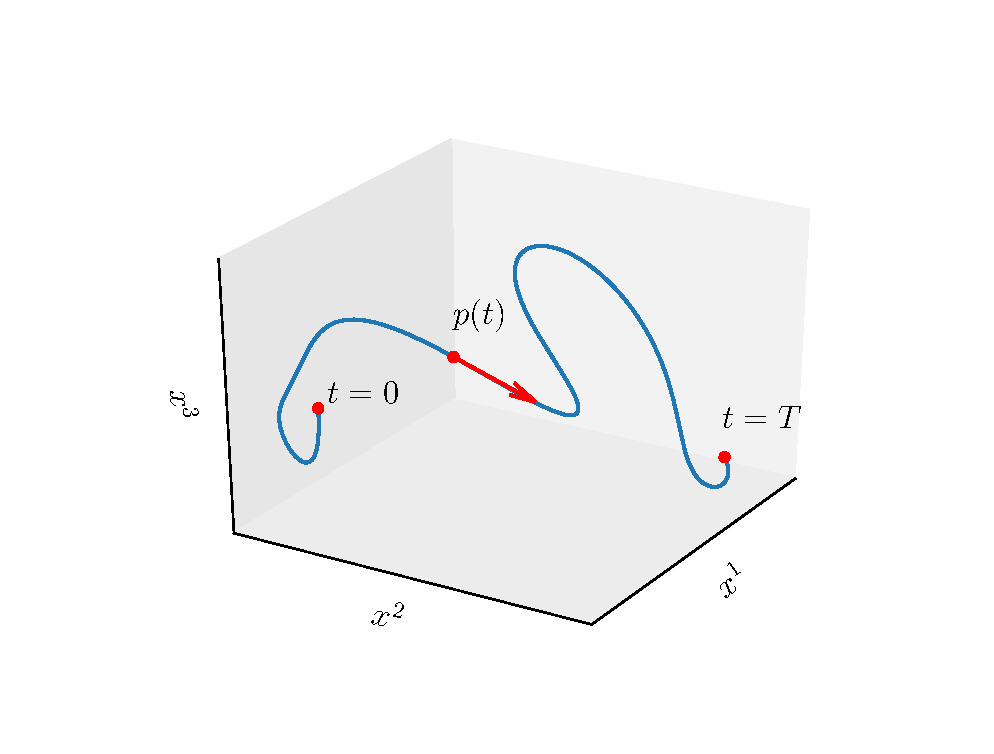
\includegraphics[scale=0.6, bb=0 0 461 346,trim={1cm 1cm 1cm 2cm},clip]{visualization.eps}
  \caption{Visualization of a smooth curve on a three dimensional
    manifold $M$ in coordinates $x^{1}$, $x^{2}$, and $x^{3}$
    corresponding to three time dependent variables $u^{1}$, $u^{2}$,
    and $u^{3}$. The values $u^{1}(t)$, $u^{2}(t)$, and $u^{3}(t)$ at
    time $t \in [0,T]$ are components of the vector tangent to this
    curve.}
  \label{fig:visualization}
\end{figure}

We further impose a restriction by assuming that this smooth curve is a
geodesic on $M$. The coordinates $x^{m}$ of the curve should then
satisfy the geodesic equations~\cite{deFelice-1990, schrodinger-1985},

\begin{equation}\label{eqn:geodesic-x}
\ddot{x}^{m} + \Gamma^{m}_{\;ab} \dot{x}^{a} \dot{x}^{b} = 0
\end{equation}

where $x^{m}(t)$ are coordinates of $p(t) \in M$, $\dot{x}^{m} =
\frac{dx^{m}}{dt}$, and $\Gamma^{m}_{\;ab} = \Gamma^{m}_{\;ab}(p(t))$
are Christoffel symbols. Note that the summation convention is in
effect. As $u^{m}$s are components of a tangent vector with respect to
basis $\{\frac{\partial}{\partial{x^{m}}}\}$ in $T_{p(t)}M$, we have
$u^{m}(t) = \frac{dx^{m} \circ p(t)}{dt}$, and so the geodesic
equations can be formulated in terms of $u^{m}$s,

\begin{equation}\label{eqn:geodesic}
\dot{u}^{m} + \Gamma^{m}_{\;ab} u^{a} u^{b} = 0
\end{equation}

In other words, we are proposing that our $n$ time dependent variables
satisfy equation~\ref{eqn:geodesic}. As such, we need to find a connection
on manifold $M$, and thus its corresponding Christoffel symbols in
chart $(U,x)$, such that equation~\ref{eqn:geodesic} holds. Once a
connection is fixed, equation~\ref{eqn:geodesic} subject to an
appropriate boundary condition can be solved to forecast $u^{m}(t)$
for $t \in (T, \infty)$. The choice of connection is not unique. In
fact, given that information provided by $u^{m}(t)$ for $t \in [0,T]$
corresponds to only one geodesic on $M$, the set of all connections
that behave similarly near the geodesic path are equally valid
choices.

\subsection{Existence and uniqueness of solutions to geodesic equations}
\label{subsection:existence-geodesic}

Before discussing the steps needed to compute the Christoffel symbols,
we need to ensure that a unique solution to
equation~\ref{eqn:geodesic} exists given a set of Christoffel symbols
$\Gamma^{m}_{\;ab}$.

\begin{theorem}
  Let $\frac{d\bold{u}}{dt} = f(t, \bold{u})$ be a system of ordinary
  differential equations subject to $\bold{u}(0) = \bold{u_{0}}$, and
  $f$ and its derivarives with respect to $\bold{u}$ be
  continuous. Then, there exists an $\tau \in \mathbb{R}$ such that a
  unique solution exists for $t \in [0, \tau]$.
\end{theorem}

The reader may refer to ~\cite{boyes-1990} for a proof of the above
theorem. Based on the above theorem, assuming that the term
$\Gamma^{m}_{\;ab} u^{a} u^{b}$ is smooth, existence of an appropriate
connection is guaranteed only if the time range $T$ of the time series
is smaller than $\tau$, that is only if $T$ is small enough. Similarly,
finding an appropriate connection is not a sufficient condition for
existence of a solution to equation~\ref{eqn:geodesic} for $t \in (T,
\infty)$. 

\section{Computation Steps}
\label{section:computation}

In what follows, we propose an approach for computation of an
appropriate connection.

\subsection{Constraints on Christoffel symbols}
\label{subsection:chrostoffel-constraints}

It may be useful to constrain the manifold connection by assuming
conditions on Christoffel symbols. Without any constraint, we need
$n^3 N$ parameters to represent $\Gamma^{m}_{\;ab}(p(t))$. Enforcing
constraints reduces the number of parameters and protects the model
against potential overfitting. The simplest constraint is to assume
that Christoffel symbols are constant. This is a sufficient, but not
necessary, condition for the manifold to have a constant
curvature. This is a rather strong assumption. Alternatively, one can
assume that given a chart, Christoffel symbols at each point on a
manifold are linearly dependent on the coordinates of that point. The
validity of any assumption depends on the nature of time series
variables that define the manifold.

Here on, we assume that Christoffel symbols are constant to simplify
the analysis in this preliminary study. What follows can be extended
to more complicated forms of Christoffel symbols in a straightforward
manner.

One can further constrain the Christoffel symbols by making assumptions
about the underlying metric tensor. Assuming that Christoffel symbols
are those of a Levi-Civita~\cite{deFelice-1990} connection, we have

\begin{equation}\label{eqn:gamma}
\Gamma^{m}_{\;ab} = \frac{g^{ml}}{2} ( \frac{\partial g_{al}}{\partial
  x^{b}} + \frac{\partial g_{lb}}{\partial x^{a}} - \frac{\partial
  g_{ab}}{\partial x^{l}} )
\end{equation}

where $g_{ab}$ are components of the metric tensor, and $g^{ab}$ are
the inverse components such that $g_{ab} g^{bc} =
\delta^{a}_{c}$. Because the metric tensor is symmetric we have,

\begin{equation}\label{eqn:gamma-symmetry}
\Gamma^{m}_{\;ab} = \Gamma^{m}_{\;ba}
\end{equation}

One can further assume that $g_{ab}$ is diagonal. Looking at
equation~\ref{eqn:gamma}, this assumption indicates,

\begin{equation}\label{eqn:gamma-diagonal-metric}
\Gamma^{m}_{\;ab}|_{m \ne a \ne b} = 0
\end{equation}

In the remainder of this work, it is assumed that Christoffel symbols
are constant and correspond to a Levi-Civita connection with an
underlying metric that has diagonal components in chart $(U,
x)$. These constraints reduce the number of parameters to $n(2n-1)$.

\subsection{Choice of a boundary condition}
\label{subsection:boundary-conditions}

We need to fix a boundary condition to solve the system of ODEs in
equation~\ref{eqn:geodesic}. In general, we can impose a condition at
any $t \in [0,T]$. Naturally, one may choose to impose a condition either
at $t = 0$ or $t = T$. Here on, we assume that a condition is imposed
at $t = T$, that is,

\begin{equation}\label{eqn:geodesic-bc}
u^{m}(t = T) = u^{m}_{0}
\end{equation}

What follows can be readily extended to other choices of a boundary
condition. 

\subsection{Computation of Christoffel symbols}
\label{subsection:optimization-problem}

Let us denote the actual observed values of time series by
$\hat{u}^{m}(t)$ to distinguish them from predictions $u^{m}(t)$ that
satisfy equation~\ref{eqn:geodesic}. We need to compute a set of
Christoffel symbols $\Gamma^{m}_{\;ab}$ such that solution $u^{m}$ of
equation~\ref{eqn:geodesic} is an estimation of $\hat{u}^{m}$. In
other words, we aim to determine $\Gamma^{m}_{\;ab}$ by fitting
equation~\ref{eqn:geodesic} over the known values of
$\hat{u}^{m}(t_{1})$, \dots, $\hat{u}^{m}(t_{N})$. This can be
formulated as a constraint optimization problem,

\begin{equation}\label{eqn:optimization-problem}
\min_{\Gamma^{m}_{\;ab}}
J(\Gamma^{m}_{\;ab},u^{1},...,u^{n},\hat{u}^{1},...,\hat{u}^{n})
\end{equation}

where the objective function $J$ is defined as,

\begin{equation}\label{eqn:optimization-objective-raw}
J := \frac{1}{2} \int_{0}^{T} dt \sum_{m=1}^{n} (u^{m}(t) -
\hat{u}^{m}(t))^2
\end{equation}

Note that the choice of an objective function is not unique. The above
problem is constrained to the geodesic equation~\ref{eqn:geodesic} and
boundary condition $u^{m}(t = T) = \hat{u}^{m}(T)$.

\subsection{Solution of the optimization problem}
\label{subsection:adjoint-method}

We need an optimization algorithm to solve the above problem
numerically. Most optimization algorithms need the gradient of the
objective function with respect to the optimization variables, that is
$\frac{dJ}{d \Gamma^{m}_{\;ab}}$. As the number of optimization
variables $\Gamma^{m}_{\;ab}$ is potentially large, the numerical
computation of all gradients is expensive. Here, we use an approach
which is generally referred to as the continuous adjoint optimization
method~\cite{adjoint-giles}. Using the adjoint method allows one
to compute the gradient of the objective function, constrained by a
differential equation, with respect to the optimization variables, by
solving the differential equation along with an extra differential
equation only once per optimization iteration.

Let us define $\tilde{\Gamma}^{\alpha}$ with $\alpha \in [1,n(2n-1)]
\cap \mathbb{N}$ as the unique components of $\Gamma^{m}_{\;ab}$ after
applying the constraints in
section~\ref{subsection:chrostoffel-constraints}. Here on, we consider
components of $\tilde{\Gamma}^{\alpha}$ as the optimization
variables. Now, let us add the constraint ODE to the objective function as
a penalty term~\cite{adjoint-giles}. We have,

\begin{equation}\label{eqn:optimization-objective}
J(\tilde{\Gamma}^{\alpha}) = \frac{1}{2} \int_{0}^{T} dt
\sum_{m=1}^{n} (u^{m}(t) - \hat{u}^{m}(t))^2 + \int_{0}^{T} dt v_{m}
\left( \dot{u}^{m} + \Gamma^{m}_{\;ab} u^{a} u^{b} \right)
\end{equation}

where $v_{m}$ denotes the components of the adjoint variable. These
are in fact the continuous Lagrangian multipliers used to apply the
ODE constraint. Note that as $u^{m}$s transform as components of a
tangent vector, $v_{m}$s should transform as components of a cotangent
vector to keep equation~\ref{eqn:optimization-objective} unchanged
under a coordinate transformation. As such, one can consider
$v_{m}(t)$ to be components of a cotangent vector $\boldsymbol{v}(t)
\in T^{*}_{p(t)}M$ with respect to the dual basis induced by chart
$(U, x)$.

Taking the gradient of the objective function $J$ with respect to
$\tilde{\Gamma}^{\alpha}$, integrating by parts, using
equation~\ref{eqn:geodesic-bc}, and imposing $v_{r}(t = 0) = 0$, we
get,

\begin{equation}\label{eqn:objective-gradient-intg}
\frac{d J}{d \tilde{\Gamma}^{\alpha}} = \int_{0}^{T} \left[
  \frac{df}{du^{s}} + 2 \Gamma^{m}_{\;as} u^{a} v_{m} - \dot{v}_{s}
  \right] \frac{d u^{s}}{d \tilde{\Gamma}^{\alpha}} dt + \int_{0}^{T}
v_{m} \frac{d \Gamma^{m}_{\;ab}}{d \tilde{\Gamma}^{\alpha}} u^{a} u^{b}
dt
\end{equation}

where $f = \frac{1}{2} \sum_{m=1}^{n} (u^{m}(t) -
\hat{u}^{m}(t))^2$. 

We can choose to satisfy,

\begin{equation}\label{eqn:adjoint-equation}
\dot{v}_{s} - 2 \Gamma^{m}_{\;as} u^{a} v_{m} = \frac{df}{du^{s}}
\end{equation}

with boundary condition,

\begin{equation}\label{eqn:adjoint-bc}
v_{r}( t = 0 ) = 0  
\end{equation}

Equation~\ref{eqn:objective-gradient-intg} then becomes,

\begin{equation}\label{eqn:objective-gradient}
\frac{d J}{d \tilde{\Gamma}^{\alpha}} = \int_{0}^{T} v_{m} \frac{d
  \Gamma^{m}_{\;ab}}{d \tilde{\Gamma}^{\alpha}} u^{a} u^{b} dt
\end{equation}

We can calculate the gradient of the objective function using
equation~\ref{eqn:objective-gradient}, where the adjoint variables
$v_{s}$ are calculated by solving the adjoint
equation~\ref{eqn:adjoint-equation} subject to \ref{eqn:adjoint-bc}.

As we have a method to compute the gradients of the objective function
we can use any gradient based optimization method to solve
equation~\ref{eqn:optimization-problem} subject to \ref{eqn:geodesic}
as a constraint.

\subsection{Existence and uniqueness of solutions to adjoint equations}
\label{subsection:existence-adjoint}

The adjoint equation~\ref{eqn:adjoint-equation} has a unique solution
for any range of time. The follwing theorem is relevant.

\begin{theorem}
  Let $\dot{\bold{v}} + P(t) \bold{v} = G(t)$ be a system of $n$
  ordinary differential equations subject to $\bold{v}(t_{0}) =
  \bold{v_{0}}$, where $P: \mathbb{R} \to \mathbb{R}^{n}$ and $G:
  \mathbb{R} \to \mathbb{R}^{n}$ are continuous over an arbitary
  interval $I \in \mathbb{R}$. Then, there exists a unique solution to
  the system of differential equations over $I$.
\end{theorem}

The reader should refer to ~\cite{boyes-1990} for a proof. The adjoint
equation~\ref{eqn:adjoint-equation} then has a unique solution
wherever a solution to the geodesic equation~\ref{eqn:geodesic}
exists. This means that using the adjoint approach does not impose any
further limitation beyond those by the geodesic equation.

\section{Results}\label{section:results}

As a proof of concept, the proposed model was applied to a simple
canonical problem consisting of three time dependent variables,
$u^{1}(t)$, $u^{2}(t)$, and $u^{3}(t)$. The time series were generated
by adding a random noise to three correlated smooth curves for $t_{i}
\in [0,1.2]$ where $i \in [1,120000] \cap \mathbb{N}$; the values
corresponding to $t \in [0,1]$ were used to build a model and the
remaining $t \in [1,1.2]$ were used for out of sample testing of the
forecast model.

The SLSQP optimization algorithm~\cite{numerical-optimization-2006}
was used to solve ~\ref{eqn:optimization-problem}. The objective
function gradients were computed by solving the geodesic and adjoint
ODEs as was described in section \ref{subsection:adjoint-method}. The
LSODA algorithm~\cite{petzold-1983} and an explicit Runge-Kutta method
of order 5~\cite{dormand-prince-1980} were used to solve equations
\ref{eqn:geodesic} and \ref{eqn:adjoint-equation}, respectively. Note
that the geodesic ODEs were solved subject to a boundary condition at
$t = 1$. The optimization algorithm converged to a relative error of
1.0e-3 within a few iterations. The computed Christoffel symbols
$\Gamma^{m}_{ab}$ from optimization were then used to forecast the out
of sample values for $t \in [1,1.2]$ by solving the geodesic ODEs,
again subject to a boundary condition at $t = 1$.

Figure~\ref{fig:result} shows a comparison of actual values of the
three time series to those predicted by the proposed model. The in
sample predictions, for $t \in [0,1]$, are plotted in red, and the out
of sample predictions, for $t \in [1,1.2]$, are plotted in yellow. The
model captures the trend of the time series reasonably well.

\begin{figure}[!h]

  \centering
  
  \begin{subfigure}{0.325\textwidth}
    \centering
    \includegraphics[width=\linewidth, bb=0 0 461 346, trim={0.2cm 0cm 1.5cm 1cm}, clip]{u1-t.eps}
  \end{subfigure}
  \hfill
  \begin{subfigure}{0.325\textwidth}
    \centering
    \includegraphics[width=\linewidth, bb=0 0 461 346, trim={0.2cm 0cm 1.5cm 1cm}, clip]{u2-t.eps}
  \end{subfigure}
  \hfill
  \begin{subfigure}{0.325\textwidth}
    \centering
    \includegraphics[width=\linewidth, bb=0 0 461 346, trim={0.2cm 0cm 1.5cm 1cm},clip]{u3-t.eps}
  \end{subfigure}
  
  \caption{Comparison of actual and predicted time series
    $u^{1}(t)$, $u^{2}(t)$, and $u^{3}(t)$.}
  \label{fig:result}
  
\end{figure}

Figure~\ref{fig:result-geodesic} shows the corresponding actual and
predicted geodesic curves in coordinates $x$. This is the chart map
that induces the tangent space bases which correspond to $u^{1}(t)$,
$u^{2}(t)$, and $u^{3}(t)$. Again, the in sample and out of sample
predictions are plotted in red and yellow, respectively, and the
agreement between actual and predicted curves is reasonably well.

\begin{figure}[!h]
  \centering
  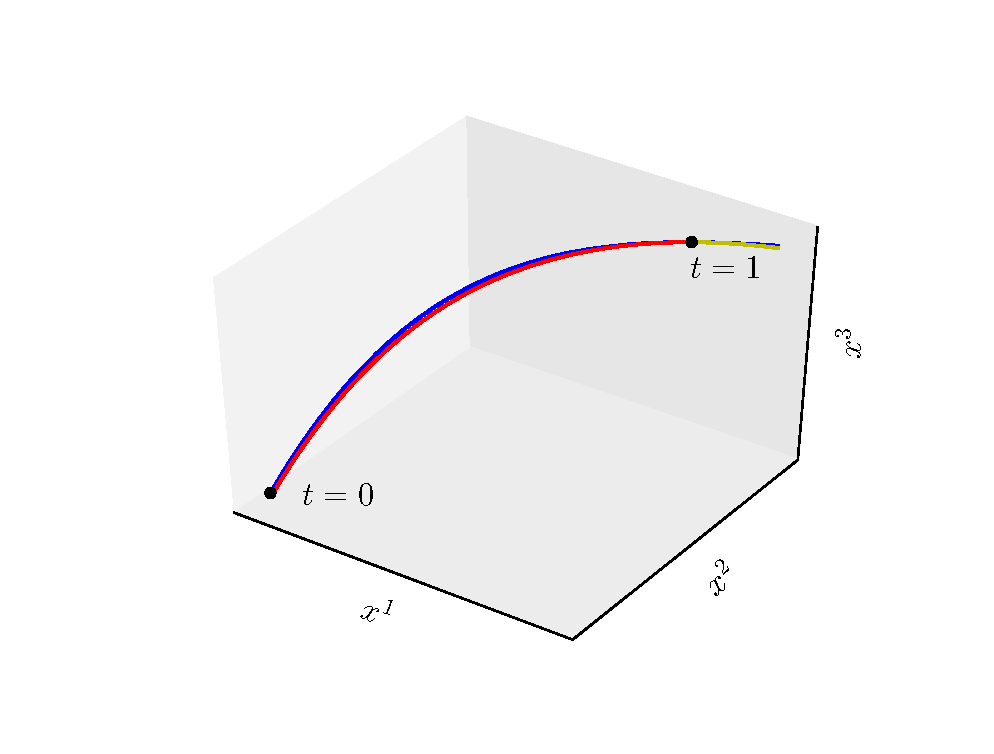
\includegraphics[scale=0.6, bb=0 0 460 345, trim={1cm 1cm 1cm 1.5cm},clip]{geodesic-result.eps}
  \caption{Comparison of actual and predicted geodesics, plotted in
    chart $(U, x)$.}
  \label{fig:result-geodesic}
\end{figure}

\section{Conclusions}\label{section:conclusions}

The present study aims at performing a proof of concept for a proposed
time series forecast model. The algorithm, under the simplifying
assumptions discussed in section
\ref{subsection:chrostoffel-constraints}, works reasonably well on a
simple canonical problem. The future work may include applying this
model to more complex problems and to relax some of the constraints in
section \ref{subsection:chrostoffel-constraints}.

%%\clearpage

\bibliography{references}

\end{document}

